%% Figure from MATH 556 notes, section 43 (Lecture 18). ADDED (not from lecture).
\begin{tikzpicture}[>=stealth]
  \begin{scope}[xshift=0cm]
    \draw[->] (0,0) -- (5.0,0) node[right, font=\scriptsize] {$n$}; \draw (0,-1.25) -- (0,1.25);
    \node[left, font=\scriptsize] at (0,1) {$1$}; \node[left, font=\scriptsize] at (0,-1) {$-1$}; \draw[gray, dotted] (0,1) -- (4.8,1); \draw[gray, dotted] (0,-1) -- (4.8,-1);
    \fill[blue!60!black] (0.24,1.000) circle (1.6pt);
    \fill[blue!60!black] (0.48,0.500) circle (1.6pt);
    \fill[blue!60!black] (0.72,0.333) circle (1.6pt);
    \fill[blue!60!black] (0.96,0.250) circle (1.6pt);
    \fill[blue!60!black] (1.20,0.200) circle (1.6pt);
    \fill[blue!60!black] (1.44,0.167) circle (1.6pt);
    \fill[blue!60!black] (1.68,0.143) circle (1.6pt);
    \fill[blue!60!black] (1.92,0.125) circle (1.6pt);
    \fill[blue!60!black] (2.16,0.111) circle (1.6pt);
    \fill[blue!60!black] (2.40,0.100) circle (1.6pt);
    \fill[blue!60!black] (2.64,0.091) circle (1.6pt);
    \fill[blue!60!black] (2.88,0.083) circle (1.6pt);
    \fill[blue!60!black] (3.12,0.077) circle (1.6pt);
    \fill[blue!60!black] (3.36,0.071) circle (1.6pt);
    \fill[blue!60!black] (3.60,0.067) circle (1.6pt);
    \fill[blue!60!black] (3.84,0.062) circle (1.6pt);
    \fill[blue!60!black] (4.08,0.059) circle (1.6pt);
    \fill[blue!60!black] (4.32,0.056) circle (1.6pt);
    \fill[blue!60!black] (4.56,0.053) circle (1.6pt);
    \node[font=\small, align=center] at (2.4,1.75) {test against $a = (1, \tfrac12, \tfrac13, \ldots) \in c_0$};
    \node[font=\scriptsize, align=center] at (2.4,-1.75) {$\langle a, e_n \rangle = \frac1n \to 0$};
  \end{scope}
  \begin{scope}[xshift=6.2cm]
    \draw[->] (0,0) -- (5.0,0) node[right, font=\scriptsize] {$n$}; \draw (0,-1.25) -- (0,1.25);
    \node[left, font=\scriptsize] at (0,1) {$1$}; \node[left, font=\scriptsize] at (0,-1) {$-1$}; \draw[gray, dotted] (0,1) -- (4.8,1); \draw[gray, dotted] (0,-1) -- (4.8,-1);
    \fill[red!70!black] (0.24,1.000) circle (1.6pt);
    \fill[red!70!black] (0.48,-1.000) circle (1.6pt);
    \fill[red!70!black] (0.72,1.000) circle (1.6pt);
    \fill[red!70!black] (0.96,-1.000) circle (1.6pt);
    \fill[red!70!black] (1.20,1.000) circle (1.6pt);
    \fill[red!70!black] (1.44,-1.000) circle (1.6pt);
    \fill[red!70!black] (1.68,1.000) circle (1.6pt);
    \fill[red!70!black] (1.92,-1.000) circle (1.6pt);
    \fill[red!70!black] (2.16,1.000) circle (1.6pt);
    \fill[red!70!black] (2.40,-1.000) circle (1.6pt);
    \fill[red!70!black] (2.64,1.000) circle (1.6pt);
    \fill[red!70!black] (2.88,-1.000) circle (1.6pt);
    \fill[red!70!black] (3.12,1.000) circle (1.6pt);
    \fill[red!70!black] (3.36,-1.000) circle (1.6pt);
    \fill[red!70!black] (3.60,1.000) circle (1.6pt);
    \fill[red!70!black] (3.84,-1.000) circle (1.6pt);
    \fill[red!70!black] (4.08,1.000) circle (1.6pt);
    \fill[red!70!black] (4.32,-1.000) circle (1.6pt);
    \fill[red!70!black] (4.56,1.000) circle (1.6pt);
    \node[font=\small, align=center] at (2.4,1.75) {test against $a = (1, -1, 1, \ldots) \in \ell^\infty$};
    \node[font=\scriptsize, align=center] at (2.4,-1.75) {$\langle e_n, a \rangle = (-1)^{n+1}$: no limit};
  \end{scope}
\end{tikzpicture}
